\renewcommand{\labelenumii}{\theenumii}
\renewcommand{\theenumii}{\theenumi.\arabic{enumii}.}
\chapter{Kravspecifikation}
\section{Aktør kontekst diagram}
\begin{figure}[H]
	\centering
	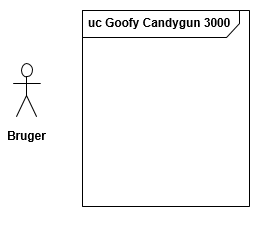
\includegraphics[]{Kravspecifikation/images/kontekstDiagram}
	\caption{Kontekst diagram for slikkanonen}
	\label{ref:kontekstDiagram}
\end{figure}

\section{Use case diagram}
\begin{figure}[H]
	\centering
	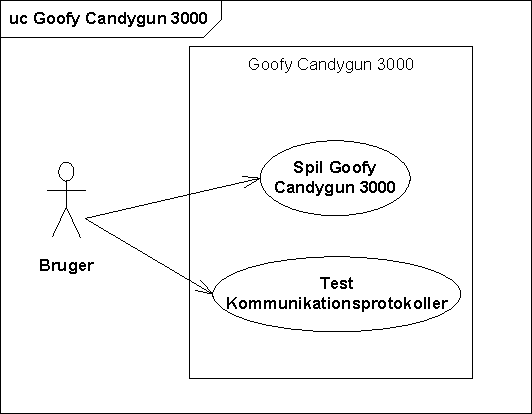
\includegraphics[]{Kravspecifikation/images/usecaseDiagram}
	\caption{Use case diagram for slikkanonen}
	\label{ref:usecaseDiagram}
\end{figure}

\section{Aktør beskrivelse}
I dette system er der en aktør, nemlig brugeren. Brugeren initierer systemet, ved at vælge spiltype på brugergrænsefladen. Derudover har brugeren mulighed for at stoppe spillet igennem brugergrænsefladen. Brugeren vil under spillet interagere med systemet gennem Wii-Nunchucken. 


\section{Fully dressed use case}
\begin{tabular}{|>{\hspace{0pt}}p{3cm}  |>{\hspace{0pt}}p{9cm}|}
	\hline
	\textbf{Navn} & Spil Goofy Candygun 3000\\ \hline
	\textbf{Mål} & At spille spillet\\ \hline
	\textbf{Initiering} & Bruger\\ \hline
	\textbf{Aktører} & Bruger\\ \hline
	\textbf{Antal samtidige forekomster} & Ingen \\ \hline
	\textbf{Prækondition} & Spillet og kanonen er operationel \\ \hline
	\textbf{Postkondition} &  Brugeren har færdiggjort spillet \\ \hline
	\textbf{Hovedscenarie} & \begin{enumerate}
		\item Bruger vælger spiltype på brugergrænseflade
		\item Bruger vælger antal skud til runde
		\item Bruger fylder magasin med slik tilsvarende antal skud
		\item Bruger indstiller kanon med analogstick på Wii-nunchuck
		\item Bruger udløser kanonen med Wii-nunchucks trigger
		\item System lader et nyt skud
		\item Brugergrænseflade opdateres med spillets statistikker
		\item Punkt 4 til 7 gentages indtil skud er opbrugt 
		\subitem [Extension 1: Bruger vælger 2 player mode] 
		\subitem[Extension 2: Bruger afslutter det igangværende spil]
		\item Brugergrænseflade viser afslutningsinfo for runden
		\item Bruger afslutter runde
		\item Brugergrænseflade vender tilbage til starttilstand
	\end{enumerate}\\ \hline
	\textbf{Udvidelser/ undtagelser} & \textbf{[Extension 1: Brugeren vælger 2 player mode]} \newline \begin{enumerate} 
		\item Bruger overdrager Wii-nunchuck til den anden bruger
		\item Punkt 4 til 7 gentages indtil skud er opbrugt
		\item Use case genoptages fra punkt 8
		\end{enumerate}
		\textbf{[Extension 2: Bruger afslutter det igangværende spil]} \newline \begin{enumerate}
		\item Brugergrænseflade vender tilbage til starttilstand
		\item Use case afsluttes
		\end{enumerate}\\ \hline
\end{tabular}

\section{Ikke funktionelle krav}
\begin{enumerate}
	\item Kanonen skal kunne drejes med en nøjagtighed på \(\pm\) 5 \(\degree\)
		\begin{enumerate}
			\item Vertikalt gælder dette for intervallet fra 0 til \(70\degree\)
			\item Horizontalt gælder dette for intervallet fra -45 til \(45\(\degree\)
		\end{enumerate} 
	\item Kanonen skal kunne affyre projektiler med en diameter på 1,25 cm \(\pm\) 2 mm
	\item Kanonen skal kunne affyre sit projektil minimum 1 meter
	\item Kanonens størrelse må maksimalt være 40cm høj, bred og dyb
	\item Fra aftryk på trigger til affyring må der maksimalt gå ti sekunder
	\item Affyring af kanonen skal kunne afvikles tre gange pr. minut
	\item Figur \ref{ref:brugergraesefladeskitse}  viser en skitse af hvordan den grafiskbrugergrænseflade kommer til at se ud
		\begin{figure}[h]
			\centering
			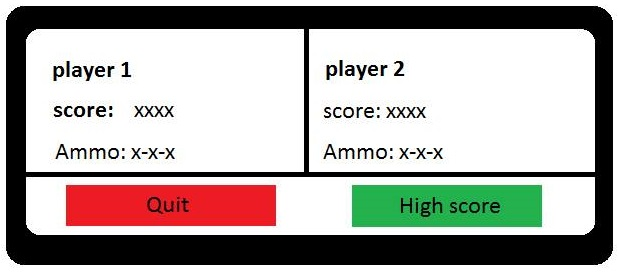
\includegraphics[width=\textwidth]{Kravspecifikation/images/brugergraensefladeskitse}
			\caption{Skitse af brugergrænsefladen}
			\label{ref:brugergraesefladeskitse}
		\end{figure}
\end{enumerate}